
% ---------------------------------------------------------------------------------------------------------------
% It is an example which *does* use the .bib file (from which the .bbl file
% is produced).
% REMEMBER HOWEVER: After having produced the .bbl file,
% and prior to final submission,
% you need to 'insert'  your .bbl file into your source .tex file so as to provide
% ONE 'self-contained' source file.


\documentclass{acm_proc_article-sp}

\usepackage{algorithm}
\usepackage{algpseudocode}
%\usepackage{amsmath}

\newtheorem{theorem}{Theorem}
\newdef{definition}{Definition}

\begin{document}

\title{GRACE: Gesture Recognition via 3D Accelerometer}


%
% You need the command \numberofauthors to handle the 'placement
% and alignment' of the authors beneath the title.
%
% For aesthetic reasons, we recommend 'three authors at a time'
% i.e. three 'name/affiliation blocks' be placed beneath the title.
%
% NOTE: You are NOT restricted in how many 'rows' of
% "name/affiliations" may appear. We just ask that you restrict
% the number of 'columns' to three.
%
% Because of the available 'opening page real-estate'
% we ask you to refrain from putting more than six authors
% (two rows with three columns) beneath the article title.
% More than six makes the first-page appear very cluttered indeed.
%
% Use the \alignauthor commands to handle the names
% and affiliations for an 'aesthetic maximum' of six authors.
% Add names, affiliations, addresses for
% the seventh etc. author(s) as the argument for the
% \additionalauthors command.
% These 'additional authors' will be output/set for you
% without further effort on your part as the last section in
% the body of your article BEFORE References or any Appendices.

\numberofauthors{3} %  in this sample file, there are a *total*
% of EIGHT authors. SIX appear on the 'first-page' (for formatting
% reasons) and the remaining two appear in the \additionalauthors section.
%
\author{
% You can go ahead and credit any number of authors here,
% e.g. one 'row of three' or two rows (consisting of one row of three
% and a second row of one, two or three).
%
% The command \alignauthor (no curly braces needed) should
% precede each author name, affiliation/snail-mail address and
% e-mail address. Additionally, tag each line of
% affiliation/address with \affaddr, and tag the
% e-mail address with \email.
%
% 1st. author
\alignauthor
Huihuang Zheng\\
       \affaddr{University of Texas at Austin}\\
       \email{huihuang@utexas.com}
% 2nd. author
\alignauthor
Yiming Pang\\
       \affaddr{University of Texas at Austin}\\
       \email{ypang@cs.utexas.edu}
}


\maketitle
\begin{abstract}
The rapid growth of various sensors on smartphones provides us with new opportunities to leverage the abundant sensor data on mobile phones to diversify user interaction based on gestures. In this report, we present GRACE: \underline{G}esture \underline{R}ecognition vi\underline{A} 3D a\underline{C}c\underline{E}lerometer. We build GRACE mainly based on the previous work of uWave~\cite{liu2009uwave}. Despite the method of dynamic time warping (DTW) used by uWave, we try to improve the performance of GRACE in the presence of fuzzy gestures by involving support vector machine (SVM). What is more, we also implement GRACE on Android phone, which can be furtherly developed to a mobile application for multiple use.
\end{abstract}


\category{Wireless Network}{Research Project}[Report]

\terms{Algorithm, Application}

\keywords{Gesture Recognition, Accelerometer, Machine Learning} % NOT required for Proceedings

\section{Introduction}
\label{introduction}
Gesture-based interactions are now widely adopted in all kinds of devices such as mobile phones, laptops and GamePads. In general, gesture-based interaction usually requires pattern recognition. Several approaches have been proposed for gesture recognition. For example, Xbox can recognize human gestures by a vision-based approach. Another category of gesture recognition is mainly based on wearable devices such as ``smart gloves'' which can detect the motion of hands. However, these approaches usually have a high requirement against computational capability and power control, which reduces the availability in daily life. In our project, we mainly focus on implementing a light-weighted gesture recognition system, which only exploits the data of 3D accelerometer, which is commonly equipped on mobile phones.

Our system GRACE is mainly built based on previous work uWave~\cite{liu2009uwave}: which is an accelerometer-based personalized gesture recognition system. uWave requires a large gesture library acting as the template. When uWave is initiated and a gesture is detected, it quantizes the acceleration data and uses DTW to compute time series Euclidean distances between the detected gesture data and predefined templates. Finally it outputs the exact template which matches the best as the recognition result. Therefore, uWave is a light-weighted system since it doesn't require high computational power or heavy training compared to the statistical methods.

In our project, we try to migrate the gesture recognition system from Wii remote to Android phone which is more widely available. We have already built the baseline of the system on an Android phone and did some experiments. On the other hand, through the experiment results, we noticed some shortcomings of uWave in the presence of fuzzy gestures and we are trying to improve the performance of the system by adopting other machine learning related methods. Our ultimate goal is to improve the performance of our gesture recognition system and build a multifunctional application on an Android phone.

The remainder of this report is organized as follows: In Section~\ref{uWave}, we discuss the work of uWave. In Section~\ref{progress} we introduce the current progress of our project followed by the future plan discussed in Section~\ref{futureplan}. Finally, we conclude our work in Section~\ref{conclusion}.

\section{uWave}
\label{uWave}
uWave mainly leverages a \textit{template library} which stores many time series of known identities for every vocabulary gesture. The basic idea of uWave is shown in Figure~\ref{uWaveBasic}.
\begin{figure}
  \centering
  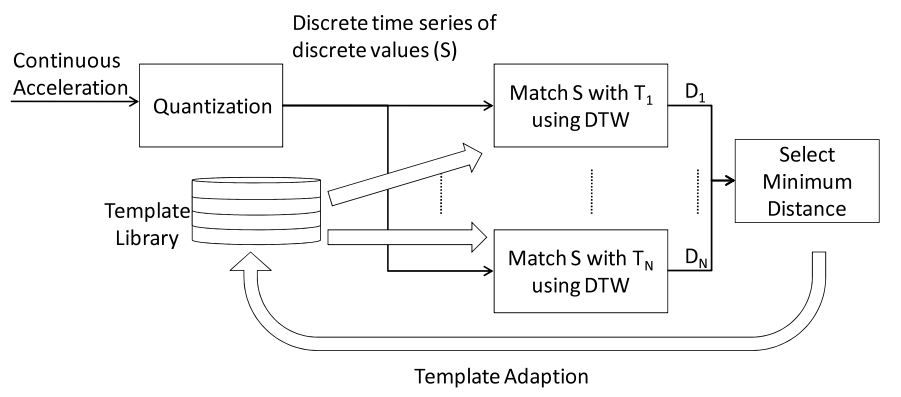
\includegraphics[width=0.8\linewidth]{uWave_basic.JPG}
  \caption{Basic idea of uWave}
  \label{uWaveBasic}
\end{figure}

When uWave is active, it takes continuous acceleration as input to a quantization module to convert the accelerometer reading into discrete values thus reduces floating point computation. The quantized data is presented as a vector of three elements, corresponding to the acceleration along the three axes. Then it will match the quantized data with data in a template library using DTW, note that the data in template library is also quantized. It then recognizes the gesture as the template that minimizes the Euclidean distance, i.e. matches the best. After the matching, the recognition result can be further used to adapt the existing templates to accommodate gesture variations over the time.

\section{Current Progress}
\label{progress}
We implemented the prototype of GRACE on Android phone based on the core of uWave. uWave is implemented in C and we transfer it to Java and encapsulate as an Android application. The current user interface is shown in Figure~\ref{GRACEui}.  
\begin{figure}
  \centering
  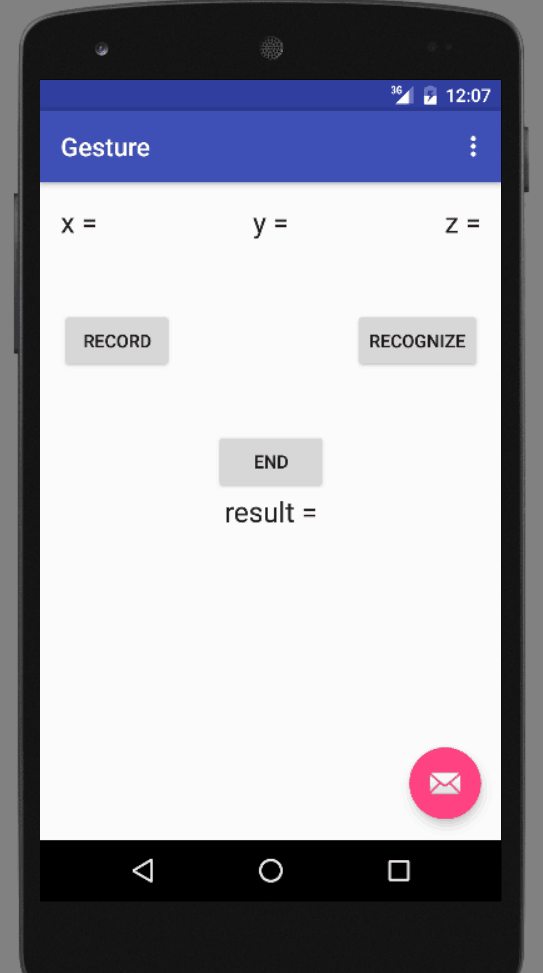
\includegraphics[scale = 0.3]{ui.png}
  \caption{Current User Interface}
  \label{GRACEui}
\end{figure} 

So far we can record the data of the accelerometer equipped on the phone and display the data along the three axes. By matching the it with existing data in the template library we can show the result of the matching gesture.

Moreover, we did some simple experiments and the results showed that the performance of GRACE is satisfying in simple settings.

\section{Future Plan}
\label{futureplan}
We plan to improve GRACE in two ways: algorithm and application, which will be presented separately.  
\subsection{SVM based method}
For the core algorithm, we intend to employ SVM to improve the accuracy of gesture recognition. In the paper of uWave, we can easily find that the accuracy of recognition will decrease with number of gestures grows. It reveals the shortcoming of uWave in the presence of fuzzy gestures. With more gestures added into the template library, some gestures can be similar to each other. In such a scenario, using distance as the metric can be highly unreliable. We can illustrate the result in Figure~\ref{SVMuWave}. Triangles and rectangles represent the feature data of two types of gestures. We can see that these two gestures are somehow similar. If we choose the red triangle and the red rectangle as templates, it will result in wrong classification. In such a scenario case, SVM can improve the accuracy of classification. Moreover, SVM can be used to ``bootstrap'' the system by classifying the templates. Therefore, involving SVM method in our system can improve the performance of the system in multiple ways.\begin{figure}
  \centering
  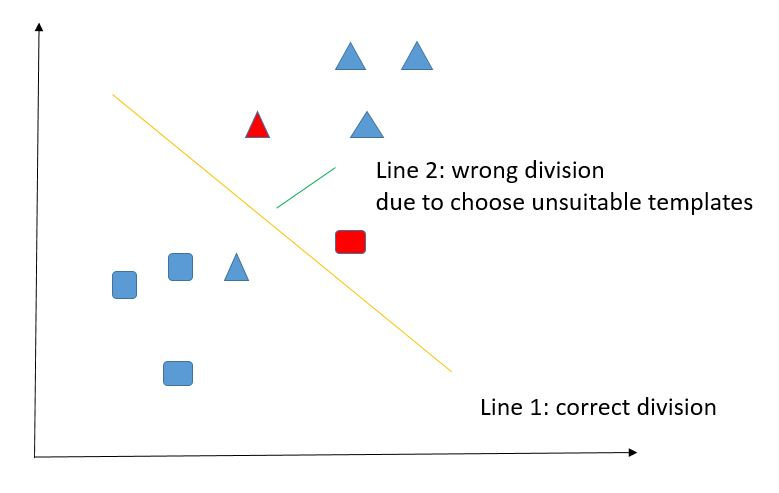
\includegraphics[width=0.8\linewidth]{SVM_better_than_uWave.JPG}
  \caption{SVM is better than uWave when we have similar gestures}
  \label{SVMuWave}
\end{figure} 
\subsection{Gesture control application}
Besides improving the core algorithm, we also want to make GRACE a useful application in gesture recognition. Since we have already built GRACE on Android mobile phone, we can easily leverage the mobile phone to develop cool applications. The application takes different gesture as input, then recognizes the gesture based on the designed algorithm. After that, the phone can execute some specific command. Our current plan is to send signals through bluetooth to a laptop and control the laptop with the phone in the air. We plan to implement the following functions:
\begin{enumerate}
  \item Control the slides with the phone: show the previous or next slide 
  \item Write directly on the slides with the phone: use the phone to write numbers (or English letters which is more challenging) and show the printed version of the writing on the slides.
\end{enumerate}

\section{Conclusion}
\label{conclusion}
In this report, we briefly introduced the work of uWave, which is an implementation of accelerometer-based personalized gesture recognition. We also present our prototype design of GRACE along with some future plans to improve the current design. We conducted several simple experiments over GRACE and showed the feasibility of GRACE in simple settings. However, the performance of GRACE in a more complicated setting is still unclear and a lot of improvements are required.


%
% The following two commands are all you need in the
% initial runs of your .tex file to
% produce the bibliography for the citations in your paper.
\nocite{*}
\bibliographystyle{abbrv}
\bibliography{sigproc}  % sigproc.bib is the name of the Bibliography in this case

% That's all folks!
\end{document}
